\documentclass[a4paper, 14pt]{article}
\usepackage{import}
\import{C:/LaTex}{pream.tex}

\title{Дискретная математика. I Семестр}
\author{Лектор: Пузынина Светлана Александровна \\
        Автор конспекта: Буглеев Антон}
\date{2022}

\begin{document}    
    \maketitle
    \newpage

    \section{Булевы Функции}
    
    \subsection*{Булевы Функции. Базис}
    \begin{definition}
        {\it Булевой функцией} называется функция вида
        \begin{align*}
            f : \{0, 1\}^n \rightarrow \{0, 1\}.
        \end{align*}
    \end{definition}

    \begin{definition}
        {\it Базис} - некоторое множество булевых функций.
    \end{definition}
    
    \begin{definition}
        {\it Формула над базисом} определяется по индукции: \\
        {\it База}: всякая функция $f \in F$ является формулой над $F$ \\
        {\it Индуктивный переход}: если $f(x_1, ..., x_n)$ - формула над $F$,
        а $\Phi_1, ..., \Phi_n$ - переменные, либо формулы над $F$, то тогда
        $f(\Phi_1, ... \Phi_n)$ - тоже формула над $F$.
    \end{definition}


    \subsection*{ПК, ДНФ, СДНФ, ПД, КНФ, СКНФ, Многочлен (полином) Жегалкина}
    \begin{definition}
        {\it Простой конъюнкцией} (ПК) называется конъюнкция одной или нескольких переменных
        или их отрицаний, причём каждая переменная встречается не более одного раза.
    \end{definition}
    \begin{definition}
        {\it Дизъюнктивная нормальная форма} (ДНФ) - дизъюнкция простых конъюнкций
    \end{definition}
    \begin{definition}
        {\it Совершенная дизъюнктивная нормальная форма} (СДНФ) - ДНФ, в которой в
        каждой конъюнкции учавствуют все переменные. 
    \end{definition}

    Аналогично определяются {\itПростая дизъюнкция} (ПД), {\itКонъюнктивная нормальная форма} (КНФ),
    {\itСовершенная конъюнктивная нормальная форма} (СКНФ).

    \begin{definition}
        {\it Многочлен (полином) Жегалкина} - сумма по модулю 2 конъюнкций переменных
        без повторений слагаемых, а также (необязательно) слагаемое 1.
        \begin{align*}
            f(x_1, ..., x_n) = a \oplus a_1 \wedge x_1 \oplus ... \oplus 
            a_{12} \wedge x_1 \wedge x_2 
            \oplus ... \oplus a_{1..n} \wedge x_1 \wedge ... \wedge x_n
        \end{align*}
    \end{definition}

    Например, $f(x, y, z) = x \oplus x \wedge y \wedge z \oplus 1$ 

    \begin{theorem}
        Для каждой функции существует единственное представление многочленом Жегалкина.
    \end{theorem}
    \begin{proof}
        \dots
    \end{proof}
    
    \subsection*{Замыкание. Замкнутые классы. Полнота}
    
    \begin{definition}
        {\itЗамыканием $[F]$} базиса $F$ называется множество всех
        функций, представимых формулой над $F$
    \end{definition}
    \begin{definition}
        {\itЗамкнутый класс} - класс, равный своему замыканию: $F = [F]$
    \end{definition}

    \begin{enumerate}
        \item $T_0 = \{f \ \vert \ f(0, \dots, 0) = 0\}$
        \item $T_1 = \{f \ \vert \ f(1, \dots, 1) = 1\}$
        \item $S = \{f \ \vert \ f(x_1, \dots, x_n) = \lnot f(\lnot x_1, \dots, \lnot x_n)\}$
        \item $M = \{f \ \vert \ \forall \text{ двоичных наборов } \alpha \leq \beta: \
        f(\alpha) \leq f(\beta)\}$
        \item $L = \{f \ \vert \ f(x_1, \dots, x_n) = x_1 \oplus ... \oplus x_n \oplus c\}$, где $c \in \{0, 1\}$
    \end{enumerate}
    
    \begin{theorem}
        Классы $T_0, T_1, S, M, L$ являются замкнутыми.
    \end{theorem}
    \begin{proof}
        \dots
    \end{proof}

    \begin{definition}
        Множество булевых функций $F$ называется {\itполной системой},
        если все булевы функции выразимы как формулы над данным базисом.
    \end{definition}

    \begin{theorem}
        Множество булевых функций $F$ является полным тогда и только
        тогда, когда $F$ не содержится ни в одном из пяти классов
        $T_0, T_1, S, M, L$. (Теорема Поста)
    \end{theorem}
    \begin{proof}
        \begin{enumerate}
            \item $\RA$ \\
            Предположим, что $F$ содержится в одном из классов $\RA$ $[F]$
            также содержится в одном из классов. Но все булевы функции не 
            исчерпываются только одним классом. Получили противоречие.
            \item $\LA$ \\
            Пусть $f_0, f_1, f_s, f_m, f_l \in F$ и $f_0 \notin T_0, 
            f_1 \notin T_1, f_s \notin S, f_m \notin M, f_l \notin L$.

            \begin{enumerate}
                \item $f_0 \notin T_0 \RA f_0(0,0,\dots, 0) = 1$. \\
                Если $f_0(1, 1, \dots, 1) = 1$, значит получена константа
                $\phi_1(x) = f_0(x, \dots, x) = 1$ \\
                Если $f_0(1, \dots, 1) = 0$, значит получено отрицание
                $\overline{\phi(x)} = f_0(x, \dots, x) = \overline{x}$

                \item $f_1 \notin T_1 \RA f_1(1, \dots, 1) = 0$. \\
                Если $f_1(0, \dots, 0) = 1$, значит получено отрицание
                $\overline{\phi(x)} = f_0(x, \dots, x) = \overline{x}$ \\
                Если $f_1(0, \dots, 0) = 0$, значит получена константа
                $\phi_0(x) = f_1(x, \dots, x) = 0$

                \item $f_s \notin S \RA \exists (\sigma_1, \dots, \sigma_n) : f_s(\sigma_1, \dots, \sigma_n) = f_s(\overline{\sigma_1}, \dots, \overline{\sigma_n})$.  
                Имея лишь отрицание из пунктов (a) и (b) мы можем получить константу с помощью
                $f_s(x^{\sigma_1}, \dots, x^{\sigma_n})$, а с помощью отрицания другую константу.

                \item $f_m \notin M \RA \exists (\sigma_1, dots, \sigma_n) : 
                \begin{cases}
                    f_s(\sigma_1, \dots, \sigma_k, 0, \sigma_{k+2}, \dots, \sigma_n) = 1 \\
                    f_s(\sigma_1, \dots, \sigma_k, 1, \sigma_{k+2}, \dots, \sigma_n) = 0
                \end{cases}$

                Таким образом, $f_s(\sigma_1, \dots, \sigma_k, x, \sigma_{k+2}, \dots, \sigma_n) = \overline{x}$, получаем отрицание.

                \item $f_l \notin L \RA$ у $f_l$ хотя бы одно из слагаемых содержит конъюнкцию.
                Расмотрим некоторую конъюнкцию. Выберем из неё два множителя $x$ и $y$. Тогда, поскольку,
                данная конъюнкция принимают единицу, $\exists$ набор $\alpha$, при котором остальные множители
                конъюнкции существуют. Тогда функция принимает вид:
                \begin{align*}
                    &f_l(x, y, \alpha) = xyp(\alpha) \oplus xs(\alpha) \oplus yq(\alpha) \oplus r(\alpha) \\
                    &f_l(x, y, \alpha) = xy \oplus xs(\alpha) \oplus yq(\alpha) \oplus r(\alpha) \\
                    &f_l(x, y) = xy \oplus xa \oplus yb \oplus c; \ a, b, c \in \{0, 1\}
                \end{align*}
                Если $a = b = c = 0$ тогда конъюнкция получена. В противном случае:
                \begin{align*}
                    &f_l(x \oplus b, y \oplus a) = (x \oplus b)(y \oplus a) \oplus (x \oplus b)a \oplus (y \oplus a)b \oplus c \\
                    &f_l = xy \oplus xa \oplus yb \oplus ab \oplus xa \oplus ab \oplus yb \oplus ab \oplus c \\
                    &f_l = xy \oplus ab \oplus c
                \end{align*}
                При любом наборе $(a, b, c)$ мы получаем либо конъюнкцию, либо её отрицание, но с помощью
                ещё одного отрицания получаем конъюнкцию. Что и требовалось
            \end{enumerate}

        \end{enumerate}
    \end{proof}

    \section{Комбинаторика}
    \subsection*{Выборки}
    \begin{definition}
        Введём $A = \{a_1, \dots, a_n\}$. Некоторый набор элементов
        $(a_{i_1}, \dots, a_{i_r})$ называется {\itвыборкой объёма $r$ из $n$ элементов} или {\it$(n,r)$-выборкой}.
    \end{definition}

    Выборки бывают {\it упорядоченные} (порядок элементов важен) или {\it неупорядоченные} (без разницы, в каком порядке элементы),
    а также {\it с повторениями} и {\it без повторений}.

    Пусть объект $A$ можно выбрать $n$ способами, а объект
    $B$ - $m$ способами. Тогда важны два правила:
    \begin{enumerate}
        \item {\it Правило суммы.} Выбор <<$A$ или $B$>> можно выбрать $n+m$ способами.
        \item {\it Правило произведения}. Выбор пары $(A, B)$ можно выбрать $nm$ способами.
    \end{enumerate}

    \begin{definition}
        Выборки $k$ элементов из $n$:
        \begin{enumerate}
            \item {\it Упорядоченная с повторениями}: $n^k$
            \item {\it Упорядоченная без повторений (размещения)}: $A^k_n = \dfrac{n!}{(n-k)!}$
            \item {\it Неупорядоченная без повторений (сочетания)}: $C^k_n = \dfrac{n!}{k!(n-k)!}$
            \item {\it Неупорядоченная с повторениями}: $\stackrel{{\wedge}}{C} = C^k_{n+k-1}$
        \end{enumerate} 
        \begin{proof}
            Пусть $A = \{a_1, \dots, a_n\}$. Неупорядоченная выборка $k$ элементов
            с повторениями задаётся вектором $(x_1, \dots, x_n)$, где $x_i$ - число повторений
            элемента $a_i$. Таким образом, $x_1 + \dots + x_n = k$

            Закодируем решение бинарным вектором $\underbrace{11 \dots 1}_{x_1} 0 \underbrace{11 \dots 1}_{x_2} 0 \dots 0\underbrace{11 \dots 1}_{x_n}$.
            Получаем вектор, состоящий из $k$ единиц и $(n-1)$ нулей. Число таких векторов: $C^k_{n-1+k}$, что и требовалось
        \end{proof}
    \end{definition}

    \subsection*{Полезные свойства сочетаний}

    \begin{theorem}
        $C^k_n = C^k_{n-1} + C^{k-1}_{n-1}$
    \end{theorem}
    \begin{proof}
        \begin{align*}
            &C^k_{n-1} + C^{k-1}_{n-1} = \\
            &\dfrac{(n-1)!}{k!(n-1-k)!} + \dfrac{(n-1)!}{(k-1)!(n-k)!} = \\
            &\dfrac{(n-k)(n-1)! + k(n-1)!}{k!(n-k)!} = \\
            &\dfrac{(n-1)!((n-k) + k)}{k!(n-k)!} = \\
            &\dfrac{n!}{k!(n-k)!} = C^k_n
        \end{align*}
    \end{proof}

    {\it Треугольник Паскаля} \dots

    \begin{theorem}
        Бином Ньютона. \[(a+b)^n = \sum_{k=0}^n C_n^k a^kb^{n-k}\]
    \end{theorem}
    \begin{proof}
        Член $a^kb^{n-k}$ участвует в разложение $(a+b)^n$ столько раз,
        сколько есть способов выбрать $a$ в $k$ множителях из $n$ - 
        а это $C^k_n$.
    \end{proof} 

    \begin{lemma}
        Грубые оценки для $n!$:
        \[(n/e)^n < n! < n^n\]
    \end{lemma}
    \begin{proof}
        Верхняя оценка очевидна. Докажем нижнюю по индукции:
        \begin{enumerate}
            \item База: $(1/e)^1 < 1 \LRA 1/e < 1$
            \item Переход: пусть верно для $n$:
            \begin{align*}
                &n! > \left(\dfrac{n}{e}\right)^n \LRA \\
                &(n+1)n! > (n+1)\left(\dfrac{n}{e}\right)^n \\
                &(n+1)! > (n+1)\left(\dfrac{n}{e}\right)^n
            \end{align*}
            Теперь покажем, что
            \begin{align*}
                &(n+1)\left(\dfrac{n}{e}\right)^n > \left(\frac{n+1}{e}\right)^{n+1} \LRA \\  
                &e(n+1)n^n > (n+1)^{n+1} \LRA \\
                &en^n > (n+1)^n \text{ (верно в курсе матанализа)}
            \end{align*}   
        \end{enumerate}
    \end{proof}

    \begin{theorem}
        Формула Стирлинга. 
        \begin{align*}
            &n! = (1 + o(1))\sqrt{2\pi n}\left(\frac{n}{e}\right)^n \LRA \\
            &\frac{n!}{1+o(1)} = \sqrt{2\pi n}\left(\frac{n}{e}\right)^n
        \end{align*}
    \end{theorem}

    % BEGINNING
    \subsection*{Язык Дика. Число Каталана}

    \begin{definition}
        {\itПравильная скобочная последовательность}. Определим по индукции:
        \begin{enumerate}
            \item пустая строка $\epsilon$ - ПСП
            \item если $w$ - ПСП, то $(w)$ - ПСП
            \item если $w, u$ - ПСП, то $wu$ - ПСП
        \end{enumerate}
    \end{definition}

    \begin{definition}
        {\it Языком Дика} называется множество всех ПСП:
        $\epsilon, (), ()(), (()), (()()) \dots$
    \end{definition}

    \begin{definition}
        {\it Числа Каталана} задаются количеством ПСП с $n$ парами скобок    
    \end{definition}
    Пример:
    \begin{enumerate}
        \item $D_0 = 1$ : $\epsilon$
        \item $D_1 = 1$ : $()$
        \item $D_2 = 2$ : $(()), ()()$
        \item \dots
    \end{enumerate}
    
    \begin{theorem}
        Рекурентная формула чисел Каталана:
        \[D_0 = 1; D_n = \sum_{k=0}^{n-1}D_kD_{n-1-k}\]
    \end{theorem}
    \begin{proof}
        Пусть $w$ - произвольная ПСП длины $2n$. Она начинается
        с открывающей скобки. Найдём ей парную закрывающуюся и представим 
        в виде: $w = (u)v$, где $u, w$ - ПСП.
        
        % ДОПИСАТЬ
        Если длина u есть $2k$, то $u$ можно составить $D_k$ способами.
        Тогда длина $v$ есть $2(n-k-1)$.   $v$ можно составить $D_{n-k-1}$ способами.
        Применим правило произведения и получим, что способов составить $D_n = D_kD_{n-k-1}$.
        Перебрав все $k$ от $0$ до $n-1$ и проссумировав получим нужный ответ.
    \end{proof}

    {\bf Числа Каталана через монотонные пути.} 

    ПСП длины $2n$ поставим в соответствие путь в квадрате $[0, n] \times [0, n]$
    из точки $(0, 0)$ в точку $(n, n)$.
        
    Открывающей скобки сопоставим горизонтальный отрезок длины $1$, а закрывающей -
    вертикальный.

    Если путь сопоставлен ПСП, то ни одна его точка не может лежать выше 
    главной диагонали квадрата.

    \begin{figure}[ht!]
        \centering
        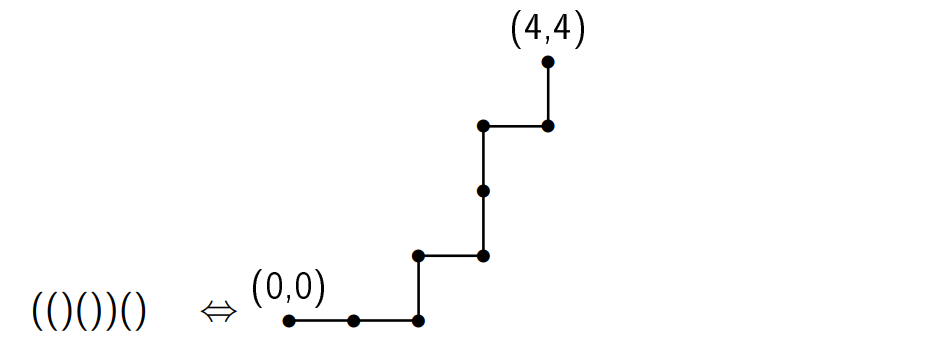
\includegraphics[width=150mm]{Capture.PNG}
    \end{figure}


    \begin{theorem}
        Аналитическая формула для чисел Каталана.
        \[D_n = \dfrac{1}{n+1}C^n_{2n}\]
    \end{theorem}
    \begin{proof}
        Сместим правильный путь на клетку вниз: теперь правильный
        путь идёт из $(0, -1)$ в $(n, n-1)$ и не имеет общих точек
        с прямой $y=x$.

        Число правильный путей $=$ общее число путей $-$ число неправильных.

        Общее число путей $= C^n_{2n}$

        Рассмотрим неправильный путь и его первую точку на 
        прямой $y=x$ - пусть это точка $A$. Отрезок до $A$ заменим
        симметричным относительно $y=x$. Получили путь длины $2n$
        из $(-1; 0)$ в $(n; n-1)$.

        \begin{figure}[ht!]
            \centering
            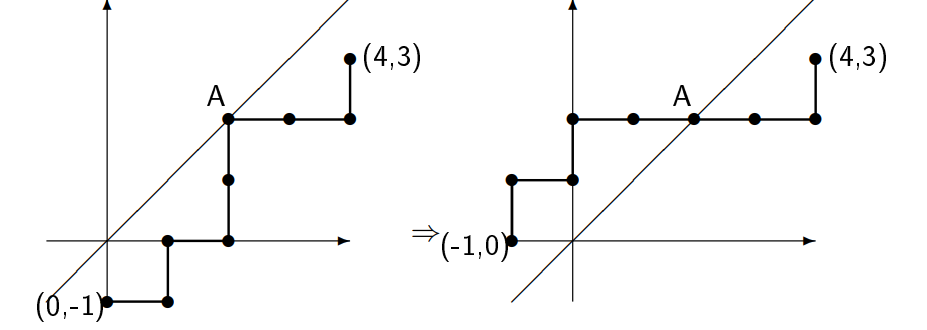
\includegraphics[width=150mm]{Capture2.PNG}
        \end{figure}

        Неправильных путей из $(0; -1)$ в $(n;n-1)$ 
        столько же, сколько и путей из $(-1; 0)$ в $(n, n-1)$.
        Учитывая, что при пути из $(-1;0)$ в $(n, n-1)$ $n-1$ вертикальных сегментов, имеем
        количество путей равное $C_{2n}^{n-1}$ 

        \[D_n = C^n_{2n} - C^{n-1}_{2n} = \dfrac{1}{n+1}C_{2n}^n\]
        %РАСПИСАТЬ
    \end{proof}

    \begin{theorem}
        Асимптотика чисел Каталана.
        \[D_n = (1 + o(1)) \cdot \dfrac{4^n}{n^{\frac{3}{2}}\sqrt{\pi}}\]
    \end{theorem}
    \begin{proof}
        Применим формулу Стирлинга. \dots
        % ДОПИСАТЬ
    \end{proof}

    \section{Графы}

    \subsection*{Много определений}
    \begin{definition}
        {\it Графом} называется пара $G = (V,E)$, где $V$ - конечное
        множество вершин, а $E \subseteq V \times V$ - множество рёбер.
    \end{definition}
    
    \begin{definition}
        Граф можно задать {\it матрицей смежности} $A = (a_{ij})$ порядка $\abs{V}$:
        \[\begin{cases}
            1, (i,j) \in E \\ 0, (i, j) \notin E
        \end{cases}\]    
    \end{definition}
    
    \begin{definition}
        Граф {\it неориентированный}, если $(u, v) \RA (v, u)$. Иначе
        граф называется {\it ориентированным}.
    \end{definition}

    \begin{definition}
        При {\itмультиграфе} допускаются кратные рёбра. Тогда в таблице смежности 
        будут присутствовать $n \in \N$.
    \end{definition}
        \begin{definition}
        Две вершины $u, v$ называются {\it смежными}, если $(u, v) \in E$.
    \end{definition}

    \begin{definition}
        Вершина $v$ и ребро $e$ называются {\it инциндетными}, если $e = (v, u)$ для
        некоторой вершины $u$.
    \end{definition}

    \begin{definition}
        Ребро, концевые вершины которого совпадают, называется {\it петлёй}    
    \end{definition}

    \begin{definition}
        {\itСтепень} deg($v$) вершины $v$ - число инциндетных ей ребёр (петля считается дважды)    
    \end{definition}

    \begin{lemma}
        \item Во всяком графе сумма степеней всех вершин равна удвоенному числу рёбер
    \end{lemma}
    \begin{proof}
        \dots    
    \end{proof}

    \begin{lemma}
        В ориентированном графе сумма входящих степеней равна сумме исходящих степеней
    \end{lemma}
    \begin{proof}
        \dots
    \end{proof}

    \begin{lemma}
        Всякий конечный граф содержит чётное число вершин нечётной степени
    \end{lemma}
    \begin{proof}
        \dots
    \end{proof}

    

    

\end{document}
